\documentclass{article}

\usepackage{polyglossia}
	\setmainlanguage{english}
\usepackage{amsmath}
\usepackage{siunitx}
\usepackage[margin=4cm]{geometry}
\usepackage{booktabs}
\usepackage{subcaption}
\usepackage{float}
\usepackage{graphicx}
\usepackage{amssymb}
\usepackage{xcolor}
\usepackage{listings}
    \lstset{language=Python,
	basicstyle=\footnotesize\ttfamily,
	breaklines=true,
	framextopmargin=50pt,
	frame=bottomline,
	backgroundcolor=\color{white!85!black},
	commentstyle=\color{blue},
	keywordstyle=\color{red},
	stringstyle=\color{orange!80!black},
	identifierstyle=\color{blue!50!green!50!black}}

\title{Computational Physics - Exercise 3}
\author{Maurice Donner \and Lukas Häffner}


\begin{document}
\maketitle
\newpage

\section{Numerov Algorithm for the Schrödinger Equation}

We implement the numerov algorithm as a 3-dimensional Vector. Like that,
we can store the Value \( y _{n+1} , y _{n} \ \text{and} \ y _{n-1} \) 
simultaneously. For each step, we store the calculated values in another array:

\begin{lstlisting}
    def numerov(x0,y_n,h,n):
    x_n = np.zeros(n)
    x_n[0] = x0
    x_n[1] = x_n[0] + h
    output = np.zeros(n)
    output[0] = y_n[0] # = y_(n-1)
    output[1] = y_n[1] # = y_n
    
    for i in range(2, n):
        x_n[i] = x_n[i-1] + h

        y_n[2] = 2 * (1 - 5/12 * h**2 * k(x_n[i-1])) * y_n[1] 
        y_n[2] -= (1 + 1/12 * h**2 * k(x_n[i-2])) * y_n[0]
        y_n[2] /= (1 + 1/12 * h**2 * k(x_n[i]))

        output[i] = y_n[2]
        y_n[0] = y_n[1]
        y_n[1] = y_n[2]

    return (x_n,output)
\end{lstlisting}

The equation to solve is the dimensionless form of the Schrödinger equation:
\[ 
    \psi ''(x) + (2 \varepsilon - x ^{2} ) \psi (x) = 0
\]

To be able to compare our results, we integrate the analytical solution into our
code. For that we need a factorial and a Hermite Polynom function:
\begin{lstlisting}
def H(x,n):
    if (n==0): return 1
    elif (n==1): return 2*x
    else: return 2*x*H(x,n-1)-2*(n-1)*H(x,n-2)

def factorial(n):
    if (n==0): return 1
    else: return n*factorial(n-1)
\end{lstlisting}

The analytical solution is:
\[ 
    \varphi (x) = \frac{H_n (x)}{(2 ^{n} n ! \sqrt{\pi} ) ^{\frac{1}{2}}} 
    \exp \bigg(-\frac{x^2}{2} \bigg )
\]
These Functions are solutions for the energy eigenvalues \( \varepsilon = n +
    \frac{1}{2}\). For the Numerov algorithm we have to differentiate between
symmetric (even \( n \) ) and antisymmetric (odd \( n \) ) solutions. For 
the symmetric solutions we have to choose \( \psi (0) = a \) and \( \psi (h) 
    = \psi (0) - h^2k_0 \psi (0)/2 \) and for antisymmetric ones \( \psi (0)
    = 0\) and \( \psi (h) = a \).
Plotting it for different orders of the Hermite Polynom \( n \) will yield:
\begin{figure}[H]
    \centering
    \begin{subfigure}{.49\textwidth}
    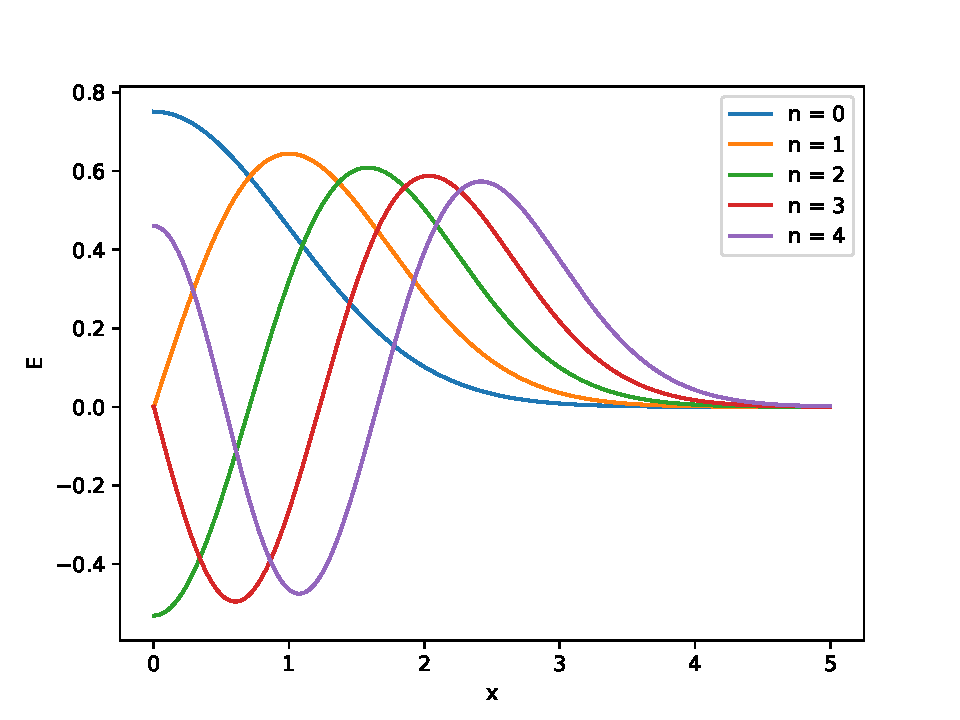
\includegraphics[width=\textwidth]{analytical.pdf} 
    \caption{Analytical Solution}  
    \end{subfigure}
    \begin{subfigure}{.49\textwidth}
    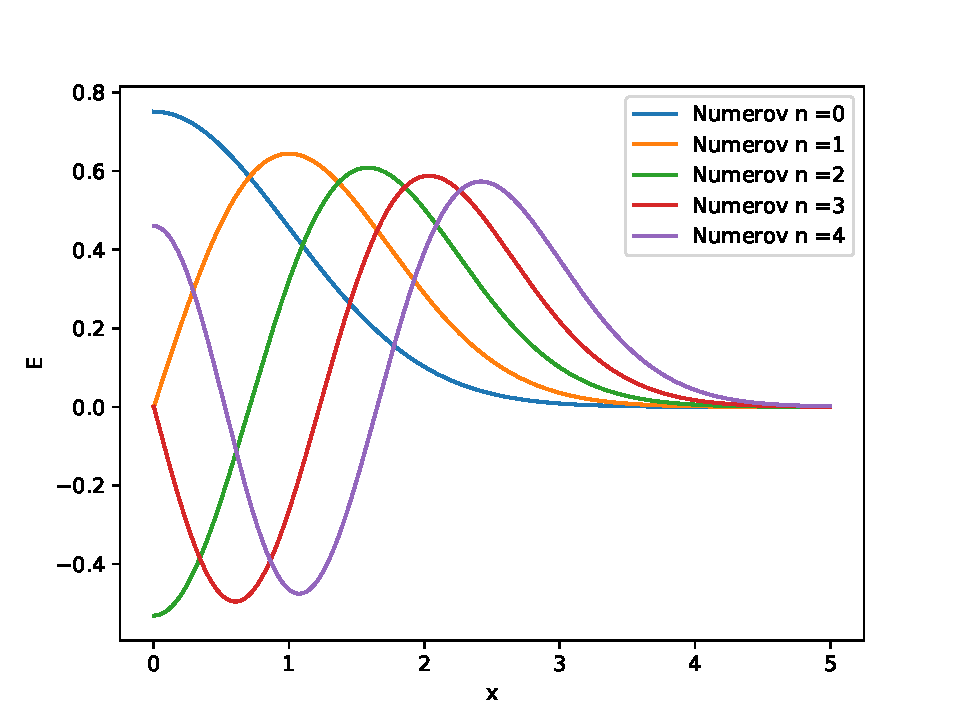
\includegraphics[width=\textwidth]{Numerov.pdf} 
    \caption{Numeric Solution}  
    \end{subfigure}
    \begin{subfigure}{\textwidth}
    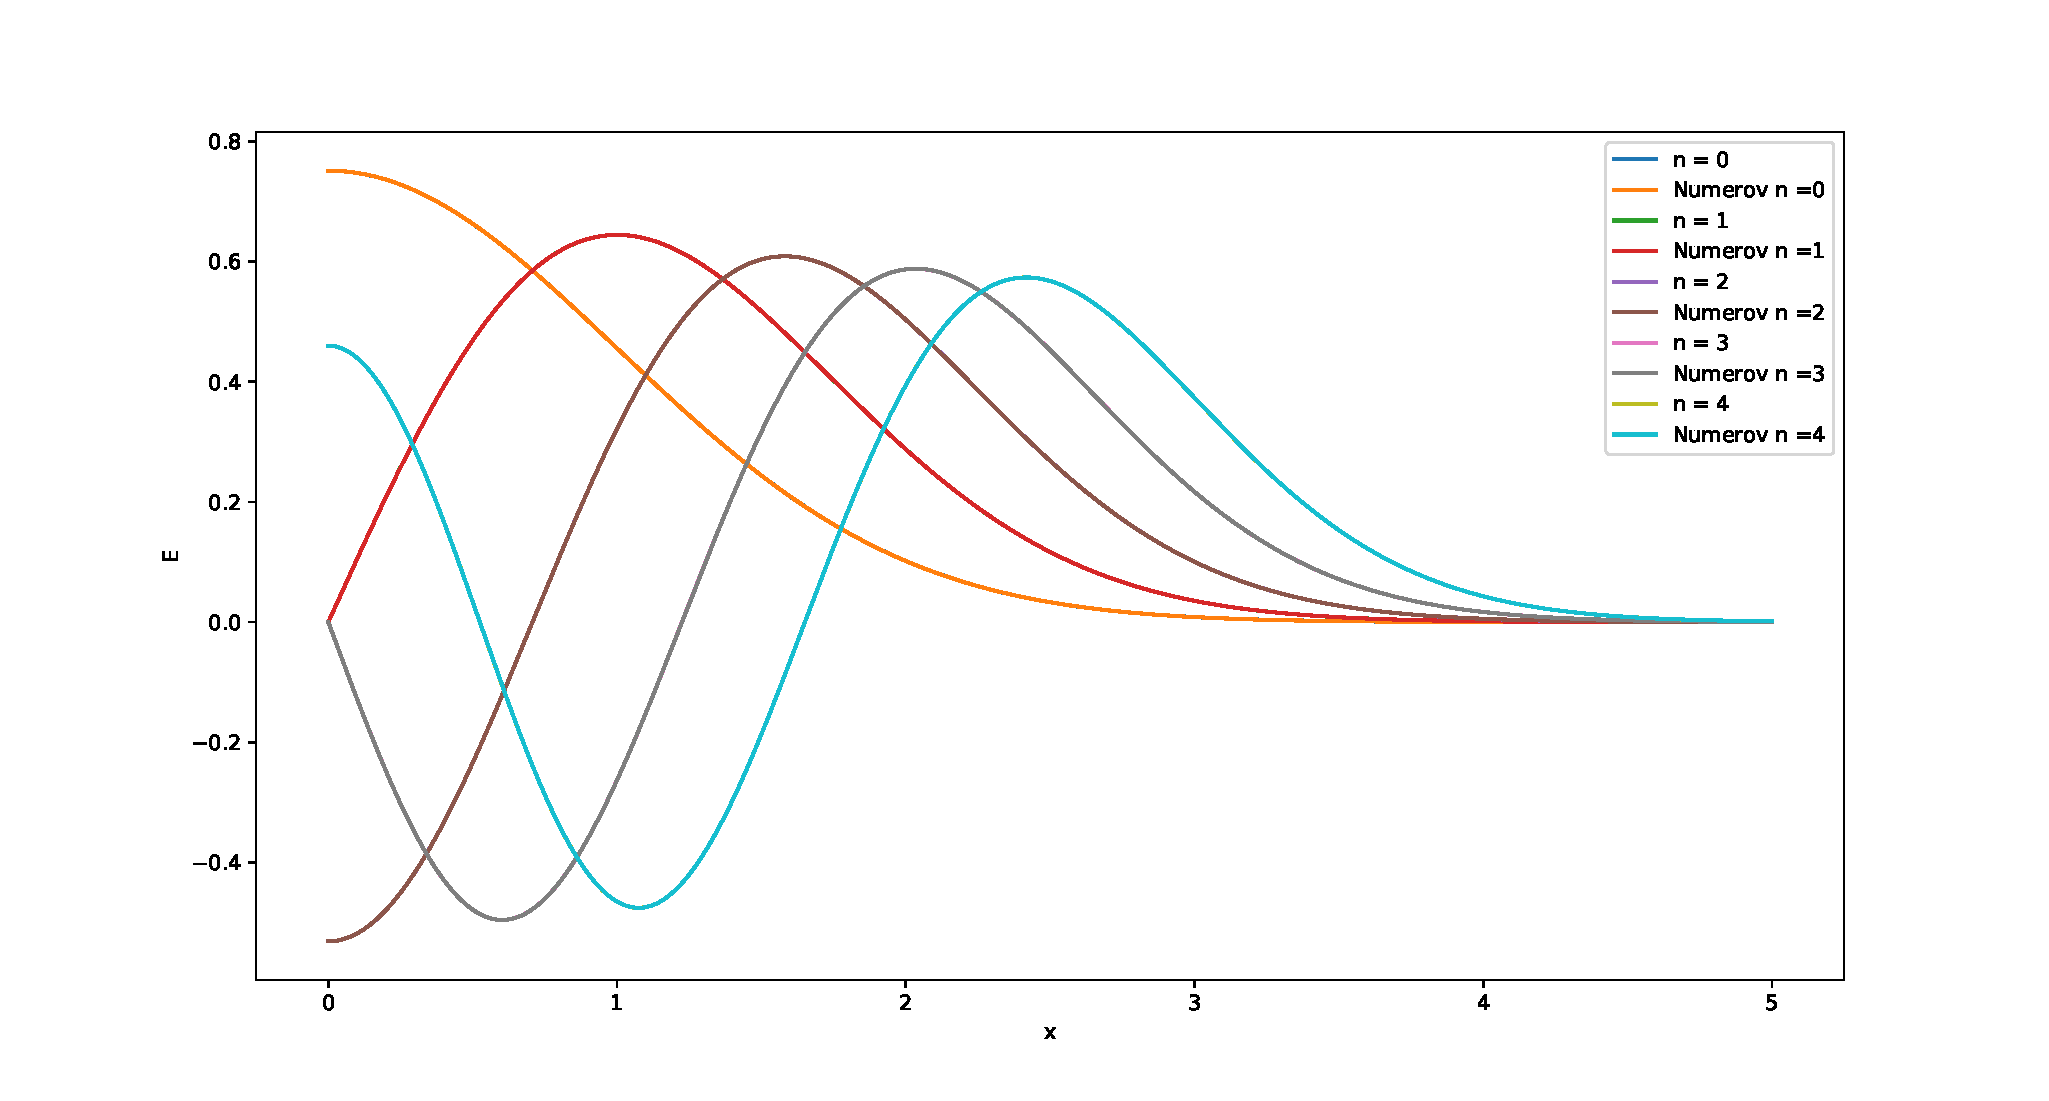
\includegraphics[width=\textwidth]{Together.pdf} 
    \caption{Overlay of Solutions}  
    \end{subfigure}
    \caption{Comparison of Solutions}
\end{figure}

As seen above, the Plot resulting from our Numerov Algortihm barely differs from
our analytical solution.

\newpage
\section*{Neutrons in the gravitational field}
We apply our Numerov Algorithm to the equation
\[ 
    \psi '' (x) + ( \varepsilon - x ) \psi (x) = 0
\]
As starting values we choose \( \psi (0) = 0 \) and \( \psi (h) = a\).
We calculate the outcome for 5 different \( \varepsilon \). From that we will take
two particularily interesting solutions (the symmetrical ones). Those solutions
with \( \varepsilon = \frac{5}{2} \ \text{and} \ \frac{9}{2}\) show similar
behaviour, except that one goes towards infinity and the other one towards
minus infinity:
\begin{figure}[ht]
    \centering
    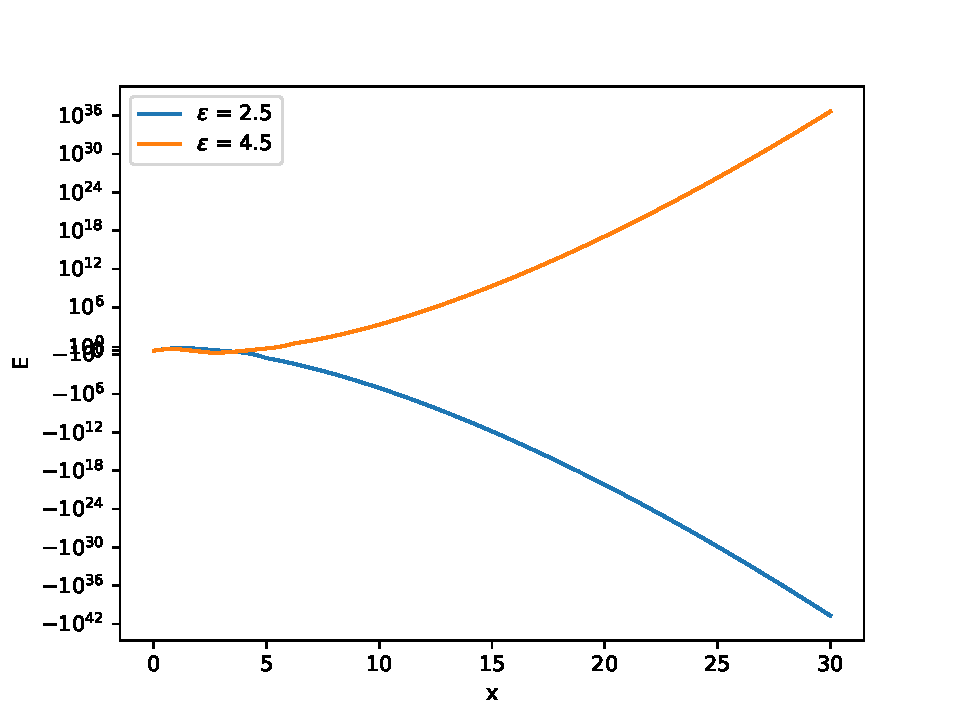
\includegraphics[width=7cm]{Neutron1.pdf} 
    \caption{Neutrons in the gravitational field for different \( \varepsilon \)} 
\end{figure}

Now we know, that at some value \( \varepsilon \), the Function changes its
sign. To find an eigenvalue, we need to find an \( \varepsilon_e \), where the
function \( \psi \) doesn't diverge, i.e. \( \psi (x) \rightarrow 0 \) for 
\( x \rightarrow \infty \). First, we roughly try to find a few values, where
the sign changes. For that, we let the program run roughly over a couple
of \( \varepsilon \) in the interval [1,10], and print the value of \( \psi (x)
\) at large \( x \) . Console output for that reads:

\begin{lstlisting}
    Testing... y = 6.280723694044417e+40 & epsilon =  2.2727272727272725
    Testing... y = -1.5235973614650188e+40 & epsilon =  2.3636363636363638
    ...
    Testing... y = -1.2707732952939073e+37 & epsilon =  4.0
    Testing... y = 2.7078206339593106e+35 & epsilon =  4.090909090909091
    ...
    Testing... y = 6.977276804418008e+33 & epsilon =  5.454545454545455
    Testing... y = -1.6852381320228214e+33 & epsilon =  5.545454545454546
    ...
    Testing... y = -1.3309549719682978e+31 & epsilon =  6.7272727272727275
    Testing... y = 4.5655959930342876e+30 & epsilon =  6.818181818181818
    ...
    Testing... y = 2.9832517516046943e+28 & epsilon =  7.909090909090909
    Testing... y = -3.0992991223435245e+28 & epsilon =  8.0
    ...
    Testing... y = -1.2773923050848915e+26 & epsilon =  9.0
    Testing... y = 2.526144567821359e+26 & epsilon =  9.090909090909092
\end{lstlisting}

Next we implement a bisection algorithm, to estimate \( \varepsilon \).
That algorithm works in the following way:
\begin{enumerate}
    \item Choose a minimum and maximum value \( ( \lambda_\text{min} ,
	    \lambda_\text{max} )\) for \( \varepsilon \)  that
	defines our interval \( [ \lambda_\text{min} ,
	    \lambda_\text{max} ] \).
    \item Cut that interval in half and set 
	\( \varepsilon = \lambda_\text{half} \).
    \item Let's assume \( \psi(x) \rightarrow - \infty \) for \( \varepsilon = 
	    \lambda_\text{min}\). We need to do the following:
    \item If \( y < 0 \) for \( \varepsilon = \lambda_\text{half} \), our new
	interval will be \( [\lambda_\text{half} , \lambda_\text{max}] \).
	Likewise, if \( y > 0 \) for \( \varepsilon = \lambda_\text{half} \),
	our new interval will be \( [\lambda_\text{min} , \lambda_\text{half}]
	\).
    \item Repeat from Step 2.
\end{enumerate}

Let's implement that method into our code:

\begin{lstlisting}
# Choose the Interval, in which you assume epsilon, and the amount of attempts
lambda_min = 2.27
lambda_max = 2.36
attempts = 100

# Check for the sign at lambda_min
x_vector, y_vector = numerov(x0,y_init,stepsize,steps,lambda_min)
sign_0 = int(np.sign(y_vector[testx]))

#start the Bisection Procedure
for n in range(attempts):     
    epsilon = (lambda_min+lambda_max)/2
    y_init=np.ndarray((3))
    y_init[0] = 0
    y_init[1] = a
    x_vector, y_vector = numerov(x0,y_init,stepsize,steps,epsilon)
    
    sign = int(np.sign(y_vector[testx]))
    
    if sign is sign_0:
        lambda_min = epsilon
    if sign is not sign_0:
        lambda_max = epsilon
print(r"Approximation for $\varepsilon$: ", epsilon) 
\end{lstlisting}

Let's choose the first example of the eigenvalue \( epsilon_e \approx 2.3 \).
We set \( \lambda_\text{min} = 2.27 \) and \( \lambda_\text{max} = 2.36 \).
With only 10 Attempts, we can calculate the Eigenvalue with an accuracy of
0.00001. If we choose to go higher, we will find the solution, where
\( \psi (x) \rightarrow 0 \) for \( x \rightarrow \infty \).
\begin{figure}[H]
    \centering
    \begin{subfigure}{.49\textwidth}
	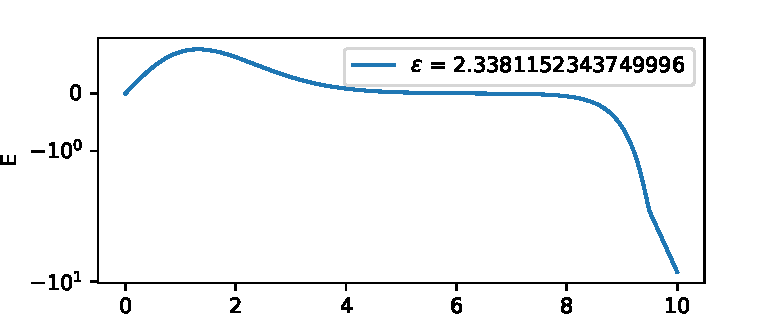
\includegraphics[width=\textwidth]{Eigenvalue_10.pdf} 
	\caption{10 Iterations} 
    \end{subfigure}	
    \begin{subfigure}{.49\textwidth}
	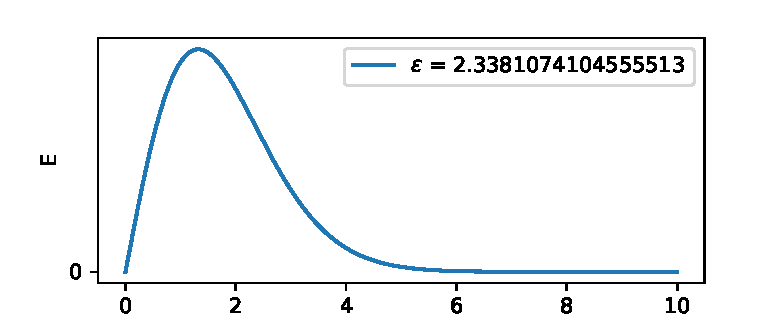
\includegraphics[width=\textwidth]{Eigenvalue_200.pdf} 
	\caption{200 Iterations} 
    \end{subfigure}	
    \caption{Determining Epsilon with a Bisection Procedure}
\end{figure}
Doing the same for the remaining \( \varepsilon _e \) up to 10, we find 6
Functions \( \psi \) with \\ \( \psi (x) \rightarrow 0 \ \text{for} \ 
x \rightarrow \infty\), together with their corresponding eigenvalues
\( \varepsilon \):
\begin{figure}[ht]
    \centering
    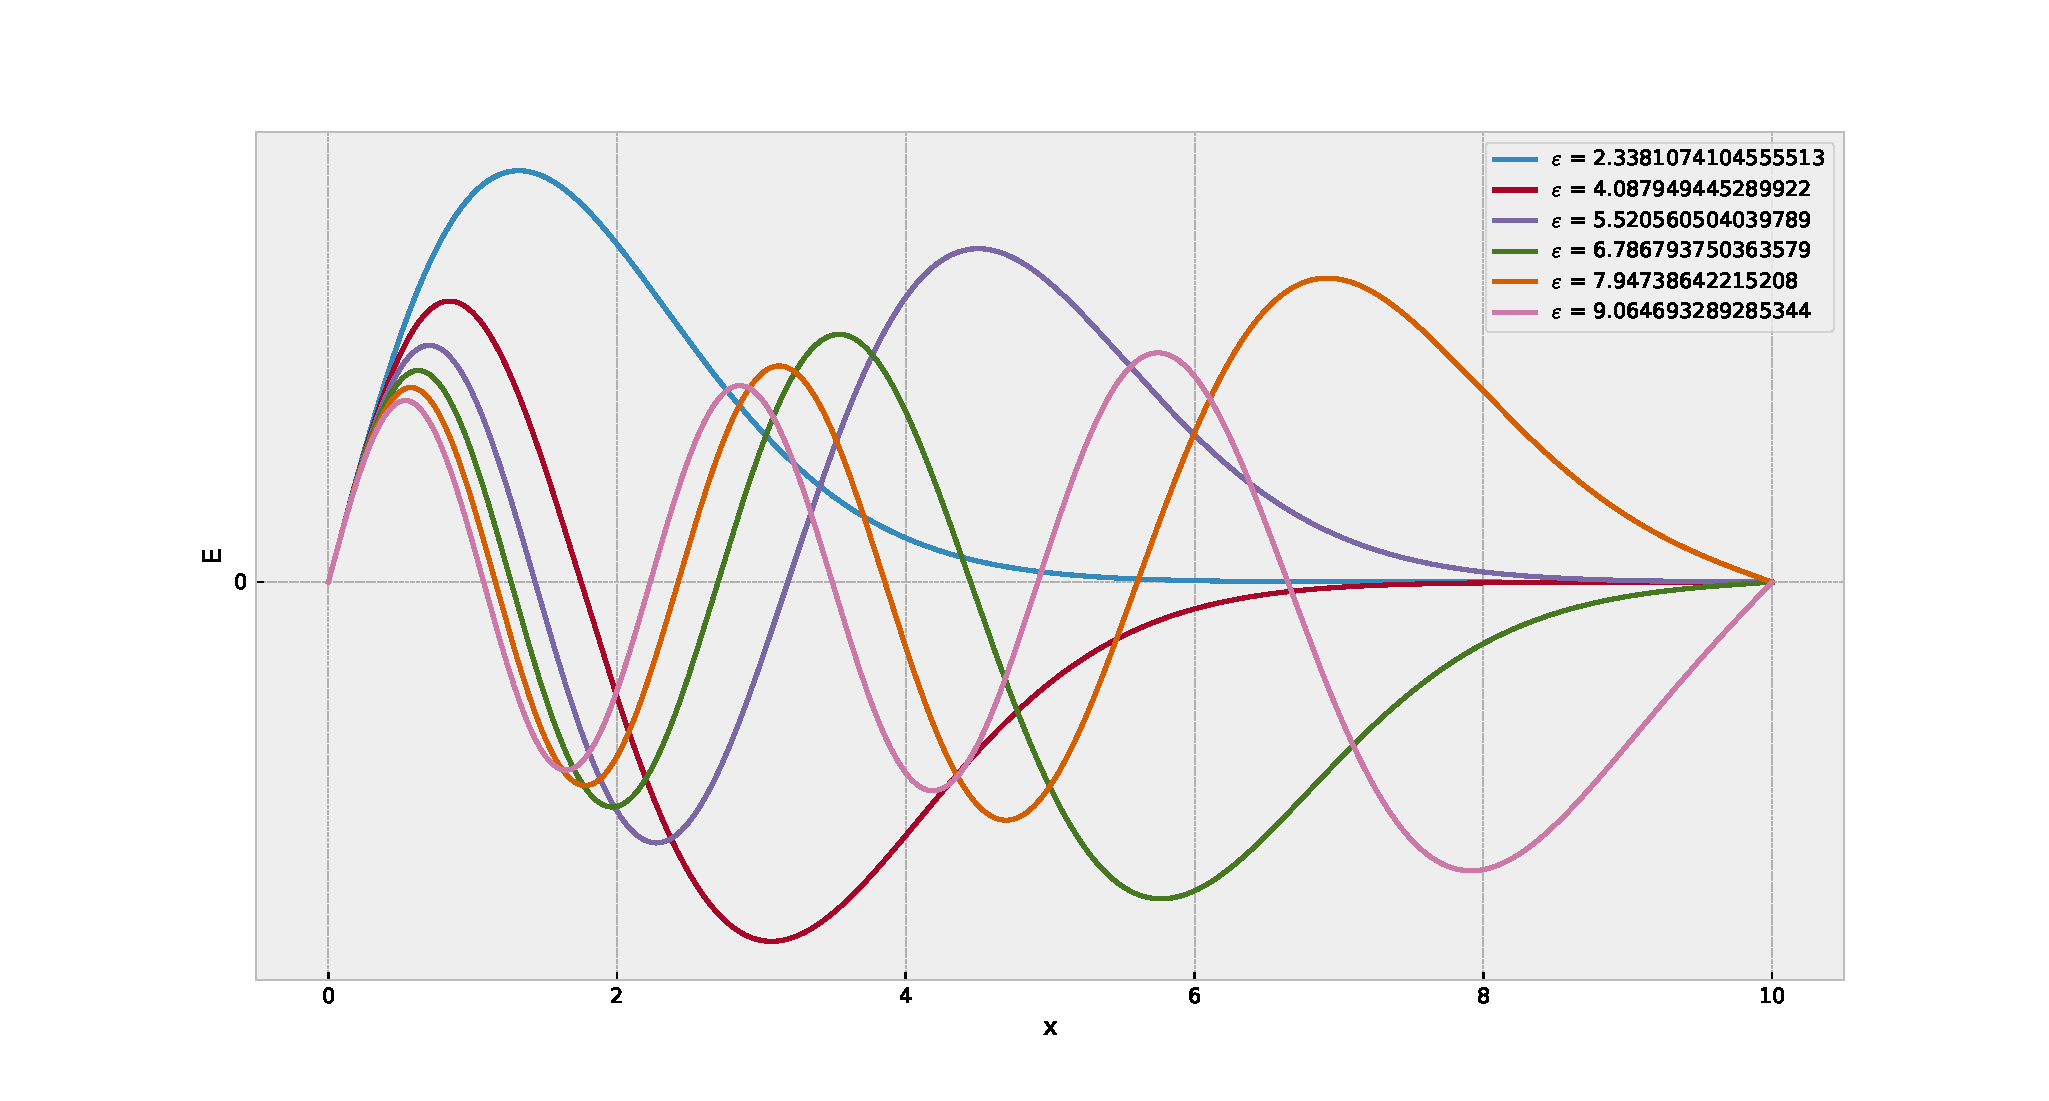
\includegraphics[width=\textwidth]{Eigenvalues.pdf} 
    \caption{The first 6 Eigenvalues $\varepsilon$} 
\end{figure}
\end{document}
